\chapter{Grundlagen und Stand der Technik}

Für den Prozess der Deformationserkennung sind grundlegende Kenntnisse der 
Additiven Fertigung sowie des 3D-Designs von Vorteil. In diesem Kapitel 
werden sowohl diese Grundlagen als auch der aktuelle Stand der Technik 
erläutert.

\section{Additive Fertigung}

Additive Fertigung (AF) ist unabhängig von dem Werkstoff ein Bereich, in dem viel
geforscht und innoviert wird. In fast jedem Industriebereich wird versucht, ein
bestehendes Design oder Modell zu optimieren und zu verbessern.
Sei es hinsichtlich Qualität oder Kosteneffizienz. AF bietet bei 
dieser Optimierung viele Vorteile gegenüber spanenden Fertigungsverfahren, da 
AF einen höheren Grad der Gestaltungsfreiheit bietet. 
AF ist eine Ressource, welche Benutzern ermöglicht, komplexe 
Bauteilgeometrien zu erstellen, ohne die Limitierung von konventionellen spanenden 
Herstellungsverfahren zu erstellen. 
Limitierungen von konventionellen spanenden 
Herstellungsverfahren kann ein hoher Materialverschleiß oder die Notwendigkeit von 
spezialisierten Werkzeugen sein.\ \cite{Vafadar.2021} 

Außerdem können mit additiver Fertigung Stückzahlen drastisch reduziert werden.
Werkstücke können bei Bedarf gefertigt werden, was die Notwendigkeit für Lagerstätten
größtenteils eliminiert. Zusätzlich können die Teile genau dort herstellt werden, wo 
sie benötigt werden, was Lieferketten und Wartezeiten verkürzt~\cite{Calignano.2023}.

Bauteile können mit verschiedenen Werkstoffen, darunter sind Polymeren, Metalle und Keramik, 
additiv gefertigt werden.
Metalle haben vor allem in den letzten Jahren 
an Relevanz gewonnen. Zusätzlich zu den schon genannten Vorteilen von AF, 
bietet Metall als Werkstoff großen Nutzen in der Industrie. Gegenüber Kunststoffen
produziert Metall weniger Abfall und kann eine höhere Qualität gewährleisten.
Zusätzlich dazu kommen die offensichtlichen Vorteile von Metall gegenüber Polymeren: 
höhere Hitzebeständigkeit und eine stabilere Grundstruktur, was sie weniger anfällig 
für Verformungen macht~\cite{Gardner.2023}.

Aufgrund dieser Vorteile wird AF in vielen Industriebereichen genutzt. Die folgende
Sektion zeigt einige Fälle in der Automobilindustrie, in denen AF 
erfolgreich benutzt wird.
Die Automobilbranche ist ein Bereich, in der AF schon viel und erfolgreich 
eingesetzt wird:
Durch AF könne Teile gefertigt werden, die leichter, belastbarer und sicherer sind. 
Die einfache Anpassbarkeit sorgt für geringe Entwicklungszeiten und Kosten. 
BWM zum Beispiel benutzt für den i8 Roadster viele AF gefertigte Teile.
Darunter sind zum Beispiel die Befestigung für das Soft-Top, die 44 \% leichter als das Spritzgussteil
ist, und dennoch zehn Mal steifer.\ \cite{Vafadar.2021} 
Fensterführungen wurden auch additiv gefertigt. Mithilfe des \glqq HP Multi Jet Fusion\grqq~
konnten 
100 Teile in 24 Stunden gefertigt werden. Selbst Teile des Zylinderkopfs für den 
S58 Motor wurden additiv gefertigt. \cite{Anusci.2019}

Auch bei älteren Fahrzeugen können additive Fertigungsmethoden zur 
Reparatur oder Restauration verwendet werden.
Gerade bei älteren Fabrikaten sind Ersatzteile häufig nicht mehr vom 
Erstzulieferer zu beschaffen oder mit konventionellen Herstellungsmethoden
wirtschaftlich herzustellen.
Bei einem Matra 530 aus 1973 wurde zum Beispiel die rechte 
Kotflügelhalterung erfolgreich reproduziert, nachdem auch nach längerer Suche
kein Originalteil gefunden wurde \cite{AMExpo365.03.06.2024}. Zusätzlich war
bei diesem Beispiel die Herausforderung, das keine digitale Version des
Bauteils existiert hat. Zuerst musste also ein Modell als Grundlage für die
additive Fertigung erzeugt werden.

\section{Limitierungen von AF}

AF kann trotz seiner Vorteile nicht überall eingesetzt werden. Limitierungen 
in der Materialvielfalt, hohe Material und Anschaffungskosten, begrenzte
Bauraumgrößen, verminderte Oberflächenqualität und aufwändige Nachbearbeitungen
können einen Einsatz von AF verhindern beziehungsweise unwirtschaftlich machen. 
\cite{inproceedings}
Einige dieser Limitierungen können umgangen oder gelöst werden. 
Zum Beispiel kann die
verminderte Oberflächenqualität kann durch eine anschließende Fräsbearbeitung
verbessert werden. 
Diese Nachbearbeitung macht eine Fixierung des Bauteils notwendig. Auch für andere
Nachbearbeitungen wie das Entfernen von Stützstrukturen kann sich das fixieren
positiv auswirken und Zeit im Herstellungsprozess eingespart werden.
Wie schon in Kapitel \ref{drawbacks_af} beschrieben, sind 
Stützstrukturen notwendig, wenn das zu produzieren Bauteil Überhänge aufweist,
die eine Steigung von ungefähr 30° unterschreiten. Der Grad des Überhangs 
variiert je nach verwendetem Material und Verfahren.

\begin{figure}[H]
    \centering
    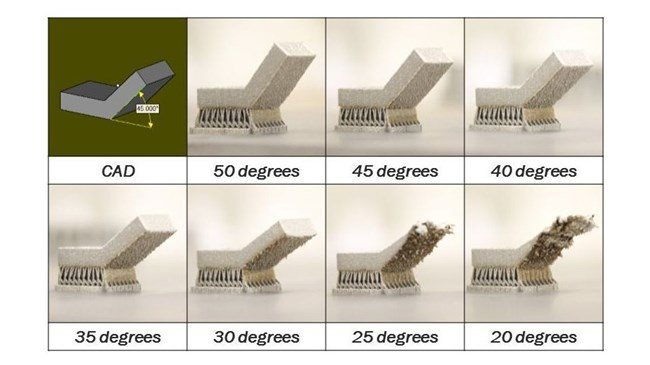
\includegraphics[width=0.9\linewidth]{images/Overhang-tests-showing-different-printabilities-and-finish-qualities-at-seven-different.jpg}
    \caption{Überhangtests mit unterschiedlichen Resultaten und 
    Oberflächenqualitäten in sieben verschiedenen Winkeln \cite{Meng.2020}}
    \label{fig:overhang}
\end{figure}

\section{Reverse Engineering}

Reverse Engineering beschreibt den Prozess aus einem bestehenden Produkt 
oder Objekt ein digitales Abbild zu erzeugen.
Dabei sind meistens wenig oder keine technischen Details über das Objekt
verfügbar.~\cite{Helle.2021}  
Auch wenn Baupläne vorhanden sind, kann es trotzdem notwendig sein, 
Reverse Engineering zu betreiben, denn das tatsächliche Produkt kann von
den Bauplänen abweichen. Produkte und Bauteile können durch die Benutzung 
abgenutzt werden und entsprechen deswegen unter Umständen nicht mehr den originalen 
Bauplänen. Zusätzlich können Toleranzen im ursprünglichen Fertigungsprozess 
für Diskrepanzen sorgen. Wenn technische Details vorhanden sind,
können diese aber im Reverse Engineering Prozess verwendet werden.\ \cite{Monchinger.2021} 
Dieses Paper zeigt, wie Reverse Engineering genutzt werden kann, um 
bestehende Bauteile passgenau zu erweitern. Konkret geht es um die
Entwicklung einer Methodik um automatisiert Laser-Scans und originale Baupläne
zusammenzufügen um ein möglichst detailgetreues Abbild der realen Struktur zu
erzeugen. Dieses Abbild wird dann benutzt, um die bestehende Struktur zu 
erweitern und auf ihr aufzubauen. Das wird am Beispiel eines Flugzeugs 
demonstriert, erst wird der Innenraum gescannt und mit dem originalen Plänen
abgeglichen, dann ein 3D Objekt erstellt. Mithilfe dieses 3D-Objekts können 
dann passgenaue Bauteile hergestellt werden, die es ermöglichen ein ehemaliges 
Passierflugzeug in eine Frachtmaschine umzubauen.
Wie schon erwähnt, wird zur erfolgreichen Weiterbearbeitung ein möglichst 
genaues digitales Abbild benötigt.
Ist dies nicht der Fall, müssen nicht passende Teile erneut hergestellt werden, 
was die Material- und Personalkosten deutlich erhöht. Es ist also im 
wirtschaftlichen Interesse beim ersten Schritt, dem Erstellen der digitalen 
Version, ein möglichst genaues Ergebnis zu erzielen. 

\section{3D Rekonstruktion}

Digitale Abbildungen von Flächen, Objekten oder sogar Körperteilen wurden in den
letzten Jahren mehr benutzt. Anwendungen sind zum Beispiel in der
geometrischen Dokumentation, Inspektion, Navigation, Visualisierung und 
Objekterkennung zu finden~\cite{Verykokou.2023}. Je nach Anwendungsfall wird eine
bestimmte Genauigkeit
der Daten erwartet, im medizinischen Bereich sind die Ansprüche natürlich ganz 
andere als zum Beispiel in der Dokumentierung von ganzen Gebirgszügen.
Das Scannen von Gesichtstexturen zeigte Abweichungswerte zwischen 140 $\mu$m und 
1330 $\mu$m, während die 3D-Rekonstruktion des Kieferknochens Werte zwischen 106 $\mu$m 
und 760 $\mu$m aufwies. 
Das Scannen eines bezahnten Bogens durch intraorale und Labor-basierte
Scanner variierte zwischen 17 $\mu$m und 378 $\mu$m und bei der 
digitalen Abtastung von Zahnimplantaten zwischen 19,32 $\mu$m
und 112 $\mu$m~\cite{Bohner.2019}.
Bei Lidar-Scans eines Sportkomplexes wurde eine Standardabweichung von ±0.10 Metern
gemessen. Es wurde aus 600 Meter Höhe vermessen und die Scandaten mit 
Referenzpunkten auf dem Boden verglichen.~\cite{Elaksher.2023}
Aus diesem Grund existieren auch verschiedene Herangehensweisen und Technologien  
zur 3D-Rekonstruktion.

3D Rekonstruktion-Technologien können in 2 Kategorien eingeteilt werden,
die bildbasierte Verfahren und die Verfahren die auf Scandaten 
beruhen.~\cite{Verykokou.2023} [TODO es existieren noch mind. 2 weitere verfahren]
Beide Verfahren können auch kombiniert werden. 
Bei bildbasierten Verfahren, auch Fotogrammetrie genannt, wird das 3D Objekt aus
mehreren zweidimensionalen Bildern erstellt, 
umso mehr Bilder vorhanden sind, desto besser kann das
3D Objekt rekonstruiert werden. Um das 3D Objekt zu erstellen werden in 
allen Bildern gemeinsame Punkte gesucht und dann mit der bekannten Kameraposition, 
die relative Position des Punktes im 3D Objekt ermittelt. Figur [todo figur einfügen] zeigt dies 
anschaulich.
Vorteil bei der Fotogrammetrie ist, dass die Daten relativ einfach aufgenommen werden
können. Die Kamera eines Smartphones kann ausreichend hochauflösende Bilder aufnehmen, um 
eine 3D-Rekonstruktion zu ermöglichen. Des Weiteren sind viele Softwarelösungen,
auch kostenlose, vorhanden um automatisiert 3D Objekte zu erzeugen.
Gründe, sich gegen den Einsatz von Fotogrammetrie zu entscheiden, 
liegen in der begrenzten Auflösung sowie im signifikant ansteigenden Arbeitsaufwand 
bei steigenden Anforderungen an die Genauigkeit des Endergebnisses. 
Fotogrammetrie zeigt jedoch ihre Stärken bei großflächigen 3D-Rekonstruktionen, 
wie sie beispielsweise bei der Erfassung von Gebäuden, Stadtteilen oder geografischen 
Strukturen erforderlich sind.

\begin{figure}[H]
    \centering
    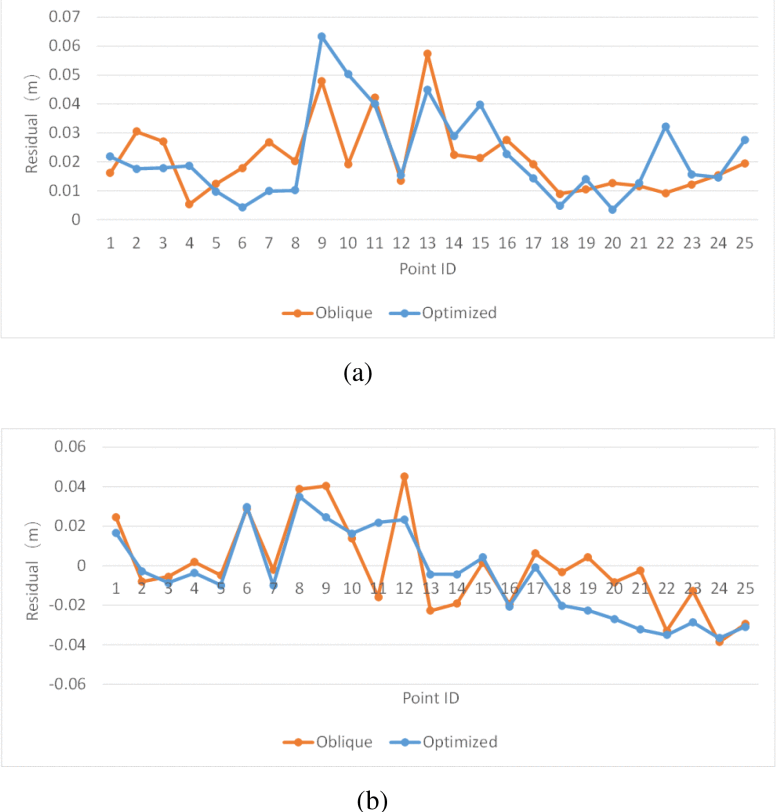
\includegraphics[width=\linewidth]{images/photogammatry_accurancy.PNG}
    \caption{Genauigkeit der Fotogrammetrie bei Bildern die aus 
    600 m Höhe aufgenommen wurden \cite{Elaksher.2023}.}
    \label{fig:photogammatryAccuracy}
\end{figure}

Für kleine Objekte, bei deren Rekonstruktion eine hohe Genauigkeit gefordert ist, 
sollte daher das zweite Verfahren angewendet werden. Bei diesem Verfahren werden
die Ursprungsdaten dreidimensional mit einem Scanner erfasst. Ein Scanner misst dabei, 
meist mithilfe von Lichtstrahlen, den Abstand zu einem Punkt auf dem zu 
rekonstruierenden Objekt. Um eine Vielzahl von Scanpunkten zu erfassen, 
wird entweder das Objekt oder der Scanner bewegt. Je mehr Punkte erfasst werden, 
desto genauer wird das Ergebnis. Allerdings nimmt die Datenmenge mit der Anzahl der 
Scanpunkte ebenfalls zu, was ab einem bestimmten Punkt zu einer Einschränkung durch den 
verfügbaren Speicher führen kann. Zudem steigt die Rechenzeit mit der Datenmenge an, 
und je nach angewendetem Verfahren kann dieser Anstieg sogar 
exponentiell sein~\cite{XiaoleiDu.2009}.

Nachteile von diesem Verfahren sind die hohen initialen Kosten eines Scanners 
und der begrenzte Messbereich. 

\subsection{Digitales Abbild}

Das schon vorhandene oder erstellte 3D Objekt muss für die weitere Nutzung
in einem geeigneten Datenformat gespeichert werden. Hierfür haben sich mehrere
Formate etabliert. Die Geometrie eines Objekts wird häufig als Sammlung von Punkten 
gespeichert. Die Oberfläche eines Objekts wird als Serie von Polygonen beschrieben. 
Der Grad des Polygons kann variieren, häufig werden Dreiecke verwendet. 
Die Genauigkeit, mit der das Polygon-Netz die gewünschte Oberfläche 
abbildet, kann gewählt werden. 
Je kleiner die Oberfläche der Polygonen ist, desto genauer wird die Oberfläche 
abgebildet. Mit kleineren Oberflächen steigt die Anzahl der zu speichernden 
Eckpunkte, was eine größere Datei zur Folge hat.
Ein in der akademischen Welt beliebtes Dateiformat für Polygon-Netze ist das 
Polygon File Format (ply).\ \cite{KentonMchenry.2008}
Das Format kann vom Nutzer beliebig angepasst werden. Eine ply-Datei beginnt mit 
einem Header in dem die Inhaltsstruktur beschrieben wird. 
Für 3D-Objekte besteht diese meistens aus X, Y und Z Koordinaten. 
Zusätzlich können weitere Informationen gespeichert werden. Das ply Dateiformat 
unterstützt standardmäßig: \glqq vertices/edges/faces, vertex colors, textures and
material \grqq ~\cite{KentonMchenry.2008}. Weitere Informationen können durch den Nutzer 
hinzugefügt werden, 
diese können dann aber unter Umständen nicht von anderen Programmen oder Benutzern
benutzt werden.
Im Dateiheader wird zu jedem Attribut auch der Datentyp festgelegt. Durch diesen 
kann die Genauigkeit und Dateigröße beeinflusst werden. Häufig werden hier Floats oder
Integer in verschiedener Bittiefe gewählt.

\begin{figure}[h]
    \centering
    \begin{minipage}{0.32\textwidth}
        \centering
        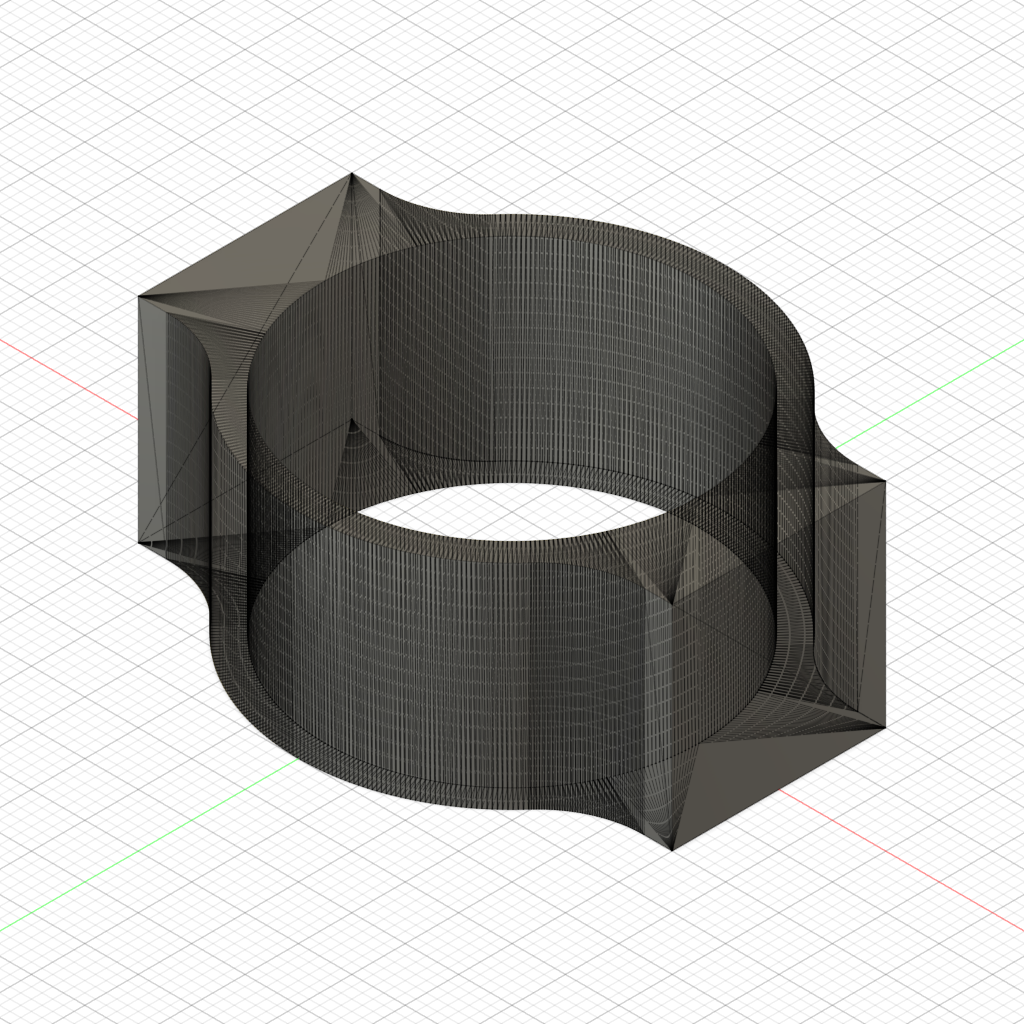
\includegraphics[width=\linewidth]{images/image_demo.PNG} % first figure itself
        \caption*{(a)}
    \end{minipage}\hfill
    \begin{minipage}{0.32\textwidth}
        \centering
        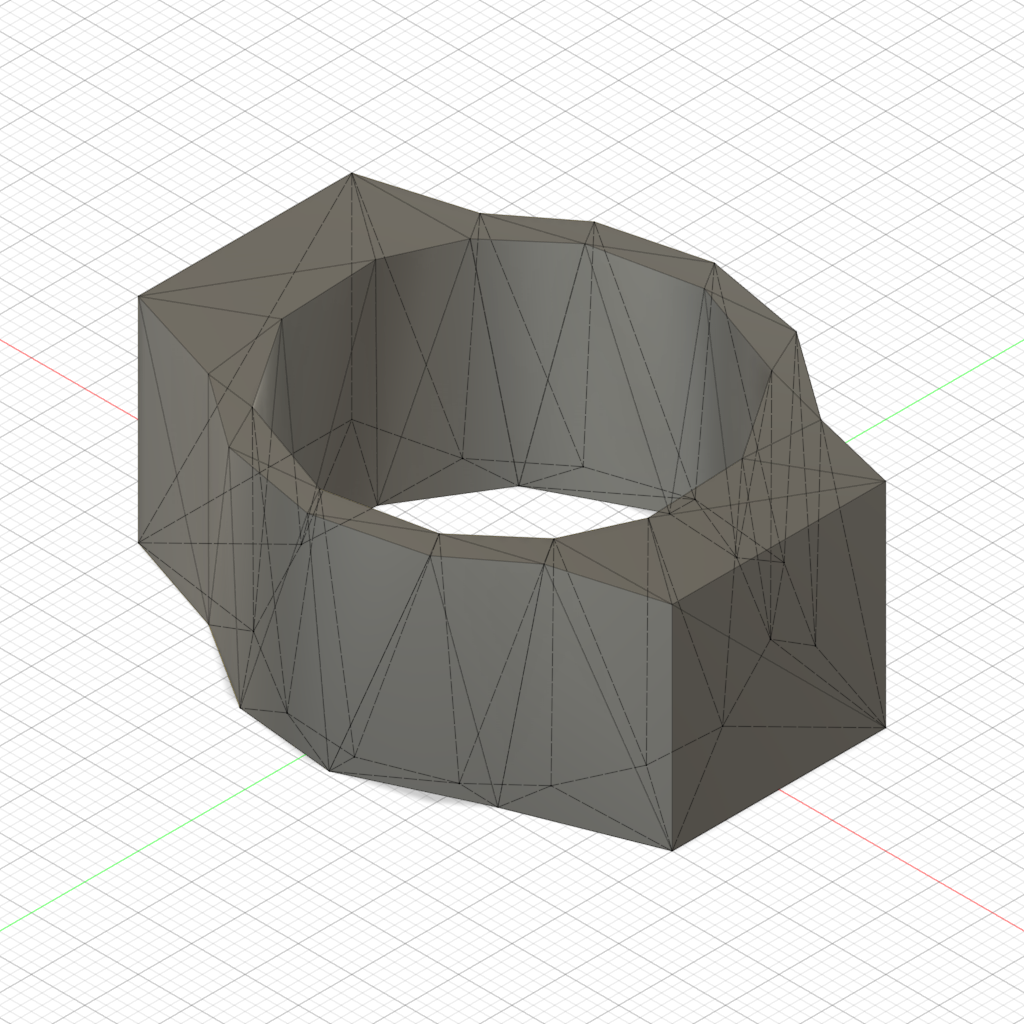
\includegraphics[width=\linewidth]{images/image_demo_medium.PNG} % first figure itself
        \caption*{(b)}
    \end{minipage}\hfill
    \begin{minipage}{0.32\textwidth}
        \centering
        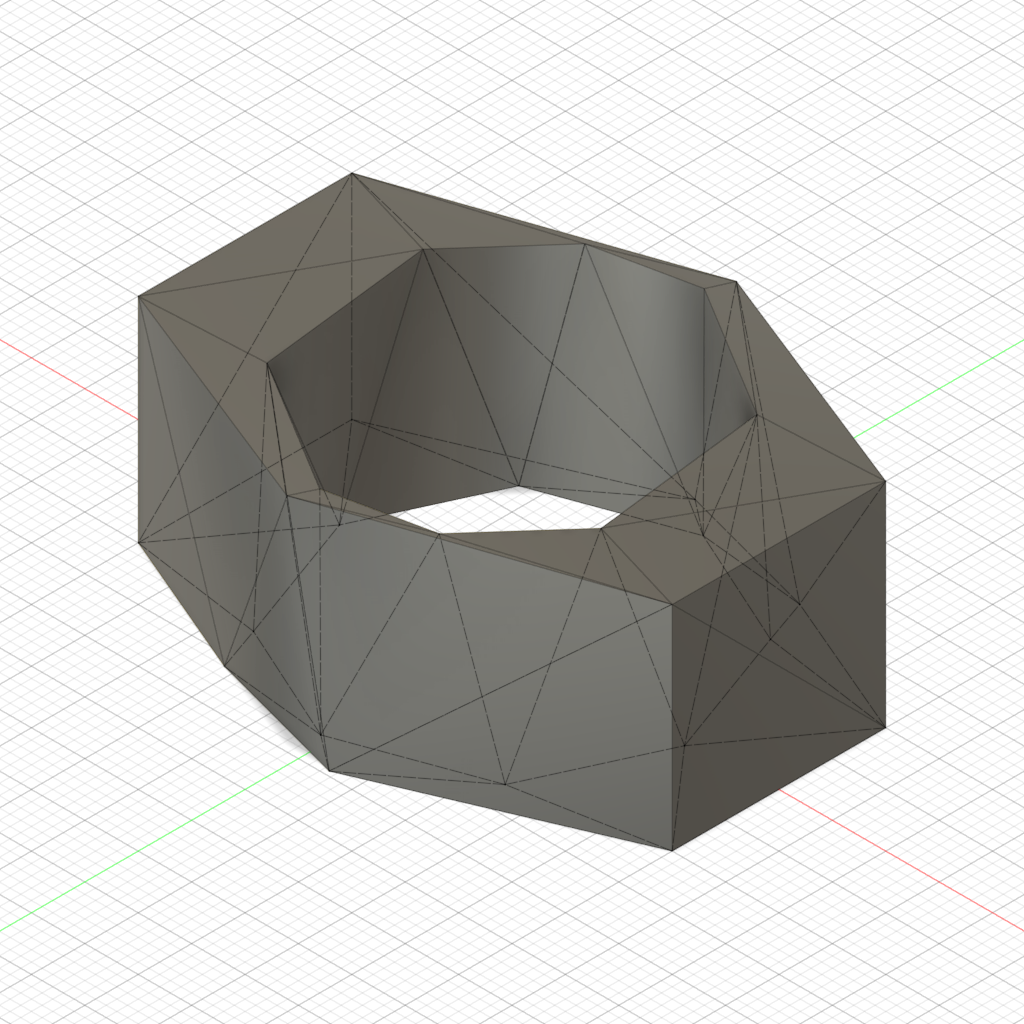
\includegraphics[width=\linewidth]{images/image_demo_low.PNG} % first figure itself
        \caption*{(c)}
    \end{minipage}\hfill

    \caption{Genauigkeit einer 3D-Datei ist abhängig von der Anzahl der gespeicherten
    Eckpunkte am Beispiel des Demonstratorbauteils. (a) 1512 Punkte
    (b) 52 Punkte (c) 30 Punkte}
    \label{fig:3d_design}
\end{figure}

\subsection{Scanner und Datenerfassung}
[todo verschiedene Scanner differenzieren und vergleichen]

Wie schon beschrieben, können dreidimensionale Daten direkt mit einem 
Scanner aufgenommen werden. 
Der Scanner hat, abhängig vom Modell und der angebrachten Höhe einen limitierten
Bereich, den er erfassen kann. 
Je nach Scannertyp und Modell kann sich der Messbereich ändern.
In Abbildung \ref{fig:scanner} ist ein Messbereich für den Scanner vom Typ 
ScanControl-LLT30xx sichtbar. Mittig kann 
in einer Tiefe von 85 mm eine Linie mit der Länge 25 mm gemessen werden. 
Der komplette messbare Bereich ist rot markiert. \cite{MESSTECHNIK_2020}
Bauteile die breiter sind als die maximale Breite der Scanebene, in Abbildung 
\ref{fig:scanner} mittig 25 mm, können also nicht in einer Pointcloud erfasst werden. 
Damit eine Digitalisierung von größeren Objekten erfolgen kann, müssen
also mehrere Scans durchgeführt, und später zusammengefügt werden. Zwischen den 
Scanvorgängen muss der Scanner in Richtung der Breitenachse verschoben werden.
Die Länge der Verschiebung sollte kleiner als die Scannerbreite sein, 
damit eine Überlappung entsteht, die 
genutzt werden kann, um die Pointclouds wieder zusammenzufügen. Die Verschiebung kann 
beliebig klein gewählt werden, jedoch steigt der Arbeitsaufwand und die Dateigröße mit 
jeder zusätzlichen Pointcloud, während das Ergebnis sich nicht verbessert.
Das Ergebnis verbessert sich nicht, da nicht mehr Daten aufgenommen werden, sondern nur 
die gleichen Daten mehrfach.
So können Pointclouds aufgenommen werden die dann in dem zu entwickelnde Verfahren
wieder zu einem digitalen Abbild zusammengefügt werden.

\begin{figure}[h]
    \centering
    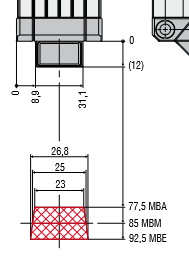
\includegraphics[width=0.3\textwidth]{images/Scanner.PNG}
    \caption{Funktionsweise eines Laserscanners [todo was ist abgebildet]}
    \label{fig:scanner}
\end{figure}

\section{Transformationen} \label{Transformation}

Eine Transformation ist eine Funktion, die eine Menge von Punkten in einem
Raum auf eine andere Menge von Punkten in demselben oder einem anderen Raum abbildet. 
Diese Transformationen werden verwendet, um die Lage, Form oder Größe von 
Objekten zu verändern.
Es gibt drei Basis Arten der Transformationen:
Translation, Rotation und Skalierung. Die Translation verschiebt alle Punkte 
um einen bestimmten Vektor in eine bestimmte Richtung. 
Rotation: Drehen eines Objekts um einen Punkt (in 2D) oder eine Achse (in 3D).
Veränderung der Größe eines Objekts durch Multiplikation der Koordinaten 
mit einem Skalierungsfaktor~\cite{XiaoleiDu.2009}.

\section{ICP-Algorithmus} \label{icp}

Der Iterative-Closest-Point-Algorithmus (ICP-Algorithmus) existiert schon seit dem Beginn der 90er Jahre und ist 
die klassische Methode, wenn es um die Registrierung von Pointclouds und 
anderen Punkt-Sets geht. \cite{icp}
Der Algorithmus errechnet eine lokale, optimale Transformation, die ein Daten-Set
dem anderen annähern kann. \cite{icp_og}
Um diese Transformation, zu bestimmen werden zuerst die Distanzen von allen 
Punkten in Daten-Set A zu dem jeweils nächsten Punkt in Daten-Set B aufsummiert 
werden. Dann wird eins der Daten-Sets verschoben und rotiert und wieder die 
Distanzen gebildet. Dies wird so lange gemacht bis die Änderung der Distanzen 
konvergiert. Die entstehende Transformation ist dann optimal.
Für identische Daten-Sets die sich nur in einer Transformation und Rotation 
unterscheiden, funktioniert dieser Algorithmus sehr gut. Bei Daten-Sets die 
Messfehler oder Überlappungen beinhalten kann häufig keine optimale 
Transformation bestimmt werden.
Deswegen wurden seit der ersten Vorstellung des Algorithmus viele Varianzen
entwickelt, die mit diesem Schwächen umgehen. 
Zum Beispiel der 'Sparse Iterative Closest Point' Algorithmus von~\cite{Bouaziz.2013}
oder die 'Anderson-accelerated' Version die besser mit Ausreißern und nur 
partiell überlappenden Daten umgehen kann und eine gleichwertige oder bessere 
Transformation errechnen kann.\ \cite{icp}
Der Algorithmus geht iterativ vor und berechnet immer eine optimale lokale Transformation.
Die beiden Daten-Set sollten schon vor dem Anwenden des ICP-Algorithmus grob angenähert sein, 
das beschleunigt die Konvergenz und damit die Laufzeit des Algorithmus.
Eine grobe Annäherung kann ermittelt werden, indem die Massenmittelpunkte der beiden Daten-Set
übereinander gelegt werden. In Abbildung \ref{fig:ipc_princip} ist das Prinzip visuell 
dargestellt. Die grünen Linien sind jeweils die kürzeste Distanz von Q nach R. 

\begin{figure}[h]
    \centering
    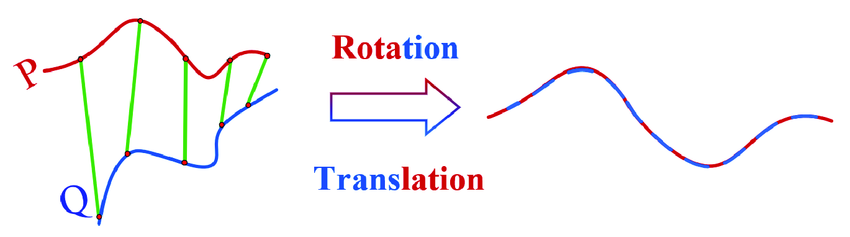
\includegraphics[width=0.3\textwidth]{images/Principle-of-ICP-algorithm.png}
    \caption{Prinzip des ICP-Algorithmus [todo größe anpassen]}
    \label{fig:ipc_princip}
\end{figure}

